\documentclass[border=10pt]{standalone}
\usepackage{pgfplots}
\pgfplotsset{compat=1.17}
\begin{document}
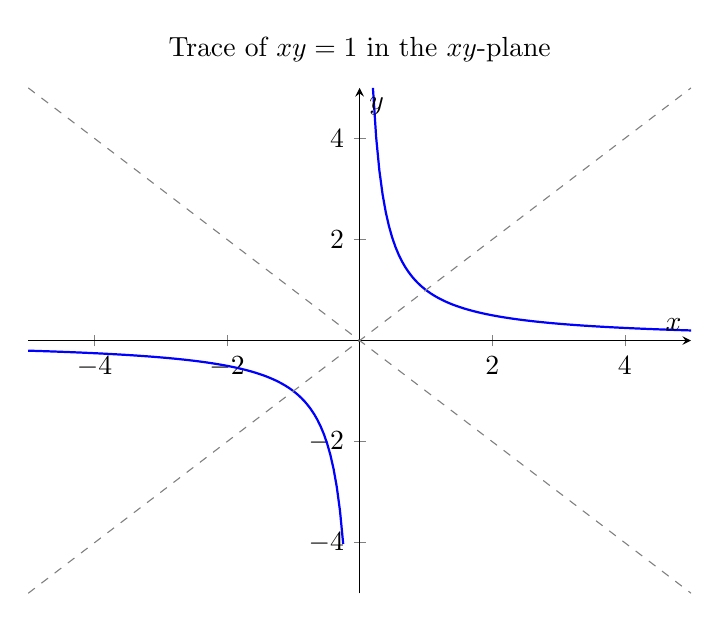
\begin{tikzpicture}
\begin{axis}[
    width=10cm, height=8cm,
    xlabel={$x$}, ylabel={$y$},
    xmin=-5, xmax=5, ymin=-5, ymax=5,
    axis lines=middle,
    samples=100,
    domain=-5:5,
    restrict y to domain=-5:5,
    title={Trace of $xy=1$ in the $xy$-plane}
]
\addplot[blue, thick, domain=-5:-0.2] {1/x};
\addplot[blue, thick, domain=0.2:5] {1/x};
\addplot[dashed, gray, domain=-5:5] {x};
\addplot[dashed, gray, domain=-5:5] {-x};
\end{axis}
\end{tikzpicture}
\end{document}
